\documentclass{standalone}
\usepackage{tikz}
\usepackage{ctex,siunitx}
\usepackage{tkz-euclide}
\usepackage{amsmath}
\usetikzlibrary{patterns, calc}
\usetikzlibrary {decorations.pathmorphing, decorations.pathreplacing, decorations.shapes,}
\begin{document}
\small
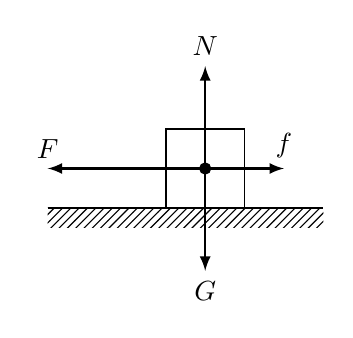
\begin{tikzpicture}[>=latex]
  % \useasboundingbox(-2.65,-1.95)rectangle(0.65,1.35);
  \draw [semithick](0.5,0) rectangle (1.5,1);
  \fill [pattern = north east lines] (-1,-.25) rectangle (2.5, 0);
  \draw [thick](-1,0)--(2.5,0);
  \draw[<->, thick] (-1,.5)node [above]{$F$}--(2,.5)node [above]{$f$};
  \draw[<->, thick] (1,-.8)node [below]{$G$}--(1,1.8)node [above]{$N$};
  \draw [fill=black] (1 ,  .5)  circle [radius=2pt];
\end{tikzpicture}
\end{document}